% !TEX root = ../maturaarbeit.tex
\chapter{Background}\label{chap:theory}
\section{Reinforcement Learning}\label{sec:RL}
\noindent
Throughout our daily lives we navigate our surroundings, handle social situations and tackle complex tasks. In doing, so we seek to take actions that based on experience or intuition we believe to have the best outcome. We might take these abilities for granted give how natural they are. However, at some point we had to obtain these skills which are so essential in managing our day to day, many through simple trial and error. Reinforcement Learning (RL) seeks to formalize this process of figuring out how to behave based on seeing what produces desirable results and what does not, and adjusting our future actions accordingly. 

\noindent
\\ Reinforcement Learning is a discipline of machine learning \cite[p. 1]{sutton_reinforcement_2018} , an incredibly broad field which is focused on the self-improvement of computer algorithms by processing data and experience. As such it is at the interface between the natural and to us intuitive concept of learning and overwhelmingly rigid and numerical world of computer programming and mathematics \cite[p. 4]{sutton_reinforcement_2018}. Thus, to be able to understand how this learning process works, and to be able to quantify and formalize it, it is essential to introduce generalizable concepts that accurately describe its components. 

\subsection*{Example: Card game UNO}\label{subsec:UNO}

\begin{figure}[ht]
    \centering
    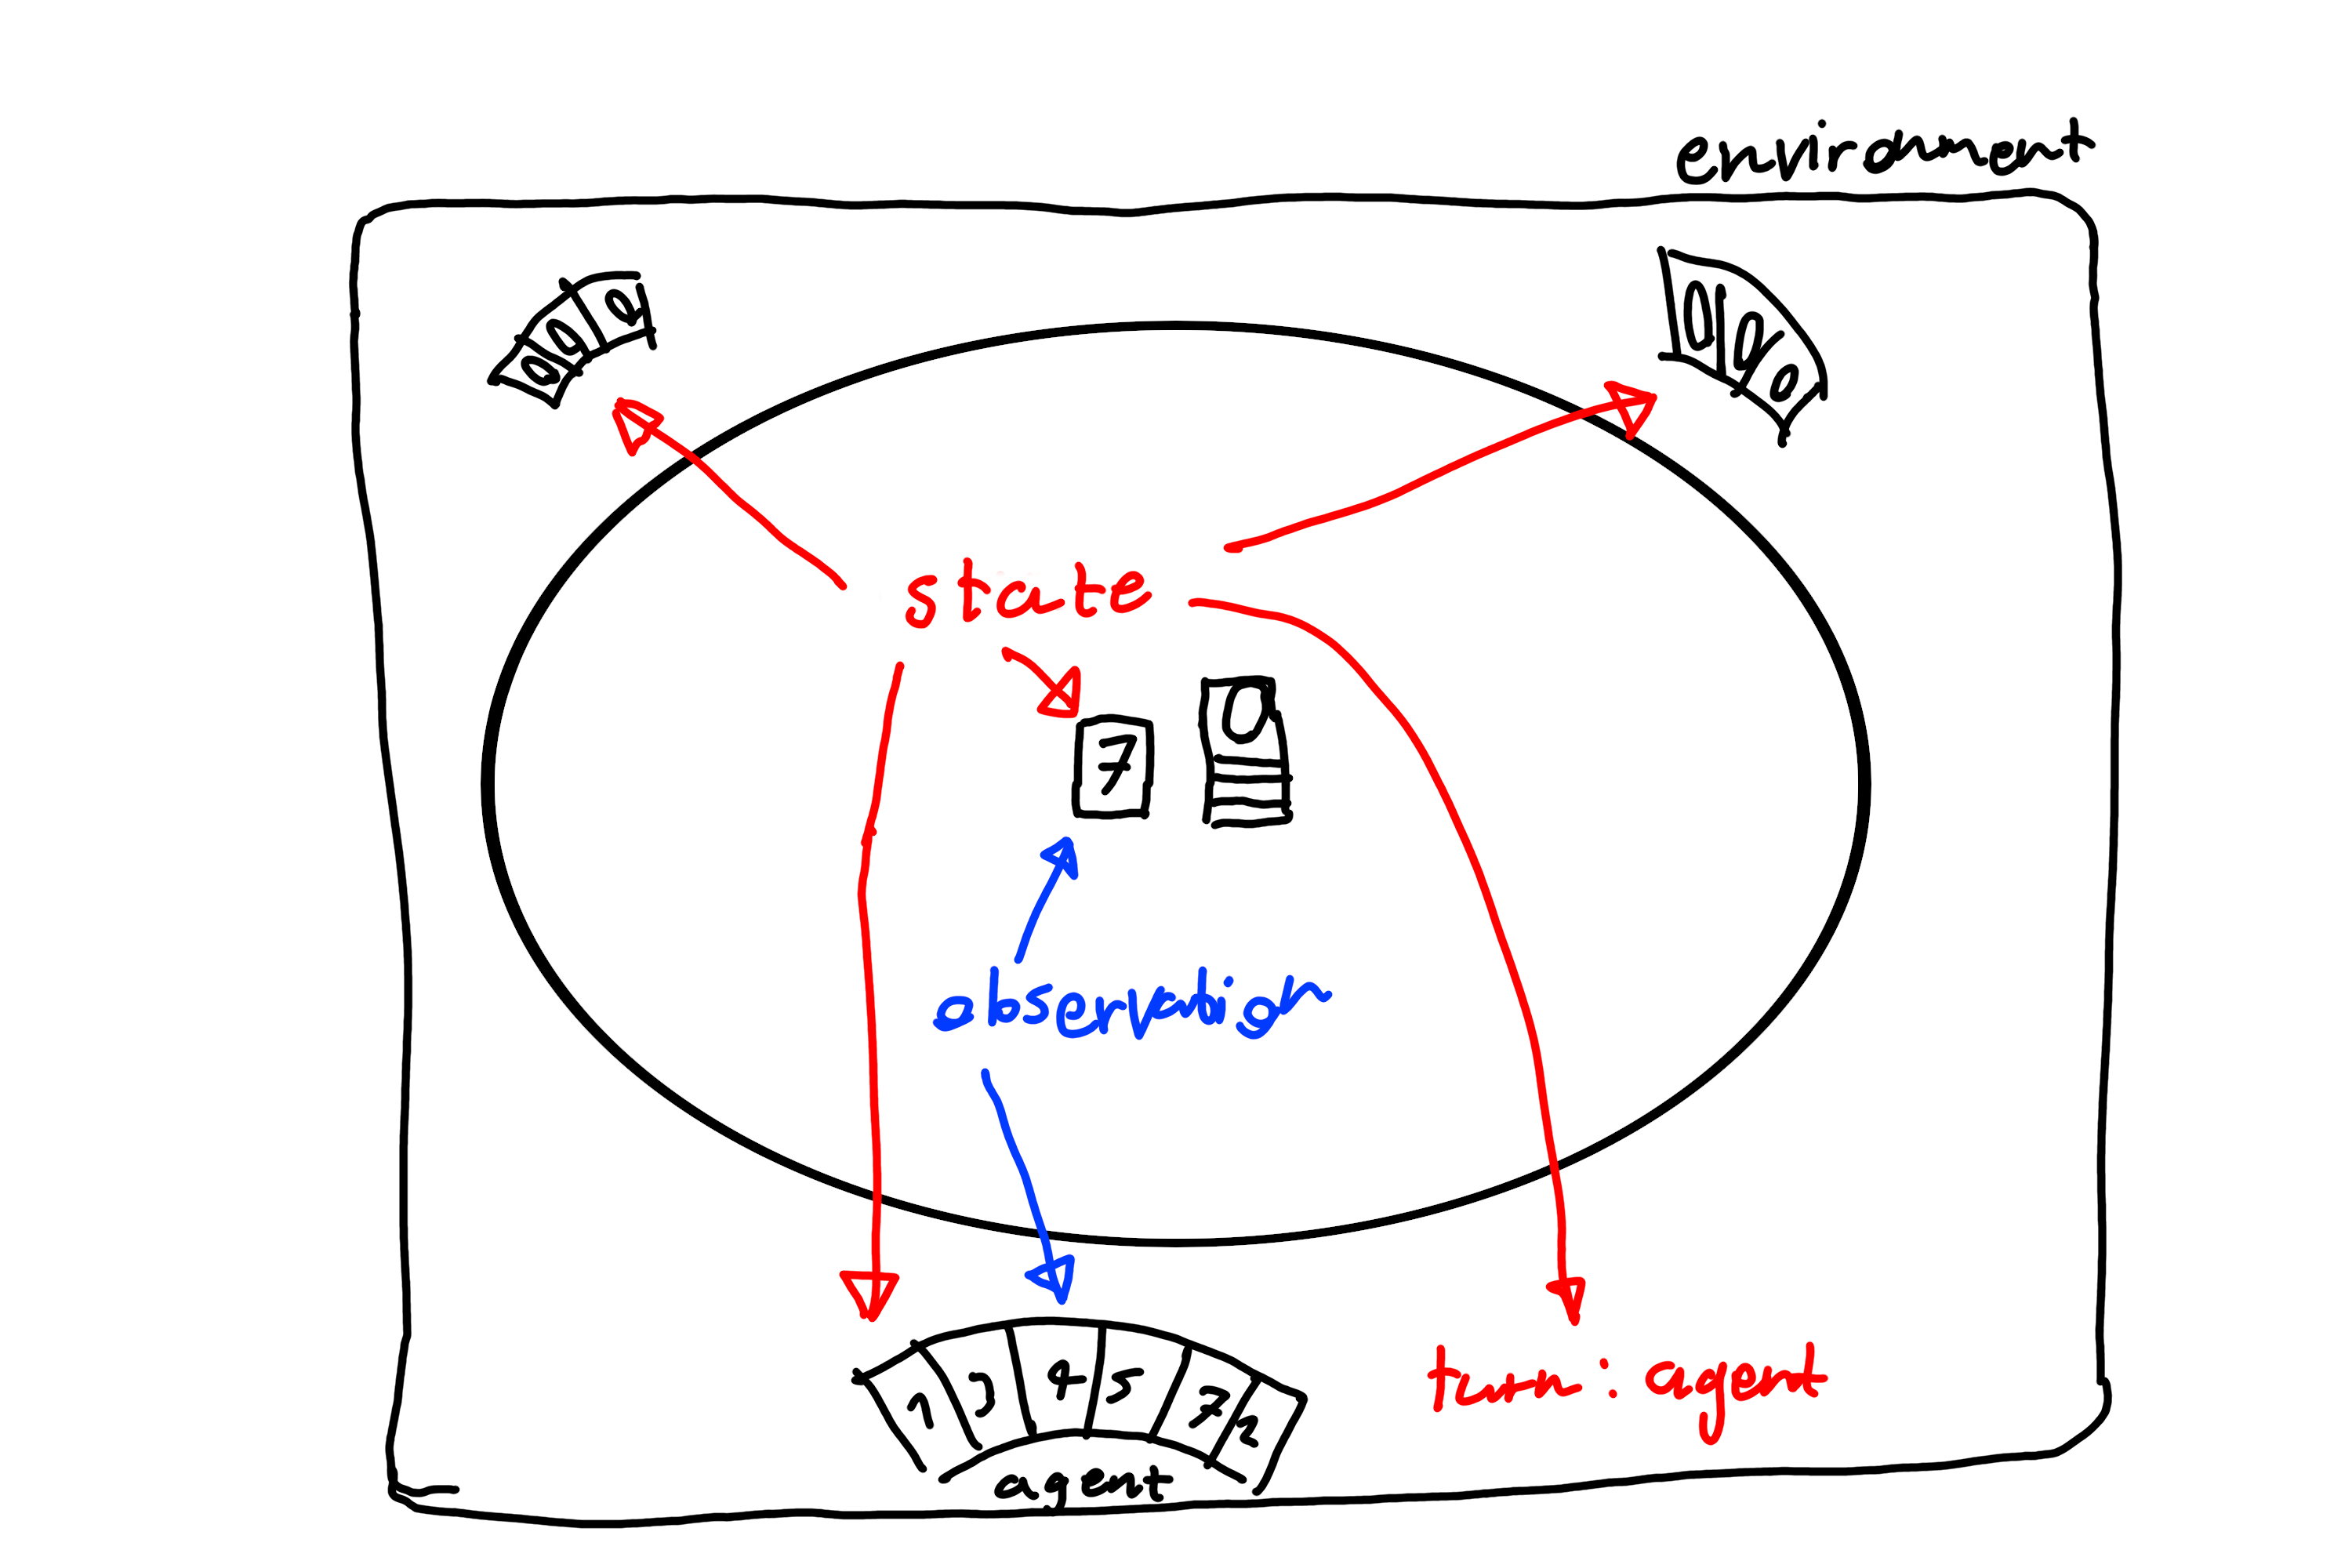
\includegraphics[width=\linewidth]{figures/UNO.png}
    \caption{UNO environment in the context of RL}
    \label{fig:UNO}
\end{figure}

\noindent
To do so, consider the example of playing the popular card game “UNO”. The \textit{objective} of the game is to rid oneself of the cards on your hand while preventing the other players from doing so. We can label the game as an \textit{environment}. This environment contains all the players, the cards and also what rules the game follows. This  can be in an any arbitrary \textit{state s}. A state of an environment describes the arrangement of all components belonging to the environment, the hands of the players, who's turn it is, what cards are on which pile and what order they are in. Notice that the environment contains a lot of information which the player which we call an \textit{agent}, an actor in the environment, does not know about. However, the actor can \textit{observe} the environment and thus gain a reasonably accurate representation of it’s state. Say it is the agents turn. Based on its \textit{observation} the agent can take an \textit{action a}, the agent can play any of the cards on its hand, or pick one up. It might not be able to play every card or none at all, and it attempting to take an action which the rules of the environment disallow will result in the same state, where it is the agents turn, but the other players will have told the agent that their action is invalid, in other words the environment will have given it a negative \textit{reward signal}. Based on the \textit{reward} the agent then can update its way of acting to produce a different action next time. The way of acting of an agent in a state given an observation of that state, is called a \textit{policy, } $\pi$. The agent can follow a policy to obtain an action.
\newline
For the sake of brevity, unless the distinction is relevant, I am going to equate observation and state moving forward. Much more expansive definitions going in to the nuances of these concepts can be found in the book \textit{Reinforcement Learning, An introduction} by Richard Sutton and Andrew Barto. \cite{sutton_reinforcement_2018}

\subsection*{Why chose Reinforcement Learning over other approaches?}\label{subsec:Why_RL}
In a simple example like UNO Reinforcement Learning might indeed not be the best approach. All the rules of UNO are known to the player, and the set of all possible states is fairly limited. The player also knows about all the cards in the game and thus an algorithm which takes in all the information available to the player, computes the card which yields the highest probability of success and chooses the action which has the highest probability of leading to victory. However, this approach requires full knowledge of how the environment operates \cite[p. 8]{sutton_reinforcement_2018}. This quickly becomes unfeasible as the environment grows more complex. Reinforcement learning lets us generate high quality solutions in uncertain environments based on a reward signal and the goal it ultimately describes \cite[p. 03]{sutton_reinforcement_2018}. Another approach which might come to mind as an obvious solution would be to simply mimic the behaviour of an optimal, or close to, agent. However, this again is impractical since such an agent might simply not exist or generating sufficient examples can be tedious. As stated in Reinforcement Learning, An Introduction: “In uncharted territory—where one would expect learning to be most beneficial—an agent must be able to learn from its own experience.” \cite[p. 02]{sutton_reinforcement_2018} Here it is important to keep in mind that uncharted environments for machines are vastly different from those of a human. There might very well be uncountable examples of brewing a coffee, but possibly non of how to power a series of motors based on a video feed in order to achieve that same goal.

\section{Markov Decision Processes}\label{sec:MDP} % NOTE: THESE ARE ALL REFERENCES TO THE BOOK
Many of the concepts introduced in \ref{sec:RL} are components of sequential decision making. Finite Markov Decision Processes (MDPs) are a formalization thereof. Environments which can be formulated as MDPs are what Reinforcement Learning is formally trying to solve. They are finite because the sets $\mathset{S}, \mathset{A}, \mathset{R}$ of all states, actions, and rewards are all finite. In an MDP the agent and environment continually interact with each other. 

\begin{figure}[h!]
    \centering
    \includegraphics{}
    \caption{Agent Environment Interaction Loop}
    \label{fig:agent_env_inter}
\end{figure}

\noindent
This interaction can be broken up in to time-steps. At each time-step the agent is given the current state of the environment and receives a reward based upon the previous state and action taken. thus at any given time-step $t$ there is a state, action and reward $S_t, A_t, R_t$ , where each of these is an element of their respective finite sets presented above. \citepg{48}. Since the agent environment interaction is sequential, a sequence, or in Reinforcement Learning a \textit{trajectory} $\tau$, arises, where each subsequent triple is of time-step $t+1$. \citepg{48}

\begin{equation}\label{MDP:trajectory}
    \Tau = S_0, A_0, R_1, S_1, A_1, R_2 \dots
\end{equation}
\centerline{\small\textit{from \citepg{48}}}

\noindent
\\ In an \ita{episodic} environment, an environment that ends at some terminal time-step $T$, any given trajectory has a respective terminal state $S_T$ and reward $R_T$. The notion of a terminal action does not make sense since the environment terminates at $T$, and the action which proceeds $S_T$ is $A_{T-1}$. Another component in the agent environment interaction are the \ita{dynamics} of the environment. An environment does not have to be \ita{deterministic} in an MPD. Concretely a given action can have multiple possible subsequent states and rewards, however the distribution of these must be well defined. This gives rise to the following set of equations:

\begin{equation}\label{MDP:prob_dist:0}
    p(s', r |s, a) \doteq Pr\{ S_t=s', R_t=r | S_{t-1}=s, A_{t-1}=a\}
\end{equation}
where 
\begin{equation}\label{MDP:prob_dist:1}
    \sum{s \in \mathset{S}}^{}\sum{r \in \mathset{R}}^{}  p(s', r |s, a) = 1 \mathrm{\ for\ all\ } s \in \mathset{S}, a \in \mathset{A}(s) 
\end{equation}
by extension the following can be deducted
\begin{equation}\label{MDP:prob_dist:2}
    r(s, a) \doteq \mathbb{E}[R]
\end{equation}

\subsection{Defining the Agents goals in an MDP}\label{subsec:goals}

We now know how an MDP operates and how the agent-environment interaction loop works on a formal level. The agent selects actions based on state information and and receives rewards as feedback for its previous action. It intuitively follows that the goal of the agent is to maximize the reward received. However based on the current model the agent changes its policy purely based on the reward it immediately receives after a give action, in other words it is only aware of the correlation between an action and its immediate consequences. Needless to say not being able to plan for long term reward presents a problem. The \ita{Return} $G$, which is defined as follows, presents one possible solution for this issue.

\begin{equation}\label{MDP:return}
    G_t \doteq R_t + R_{t+1} + R_{t+2} \dots + R_T
\end{equation}
\centerline{\small{\ita{\citepg{FINDPAGE}}}}

\noindent
\\ We can see that the return describes the sum of all rewards up until the end of the episode. This however presents some issue if the environment is continuous, since there is no final time-step. To remedy this \ita{discounting} is introduced. \citepg{FINDPAGE} The discounted return be expressed as the sum to infinity:
\begin{equation}\label{MDP:discounted_return}
    G_t = \sum_{k=t}^{\infty} R_{t+k+1} * \gamma ^k 
\end{equation}
or recursively as
\begin{equation}\label{MDP:recursive_discounted_return}
    R_{t+1} + \gamma *G_{t+2} \mathrm{\ where\ } 0 \leq \gamma \leq 1
\end{equation}
\centerline{\small{\ita{\citepg{FINDPAGE}}}}

\noindent
\\ According to \citepg{FINDPAGE} this generalization can be applied to the episodic case by defining the environment to transition from the final state $S_T$ to itself and to only ever give a reward of 0, thus not affecting the return of any given time-step in the episode. The following illustration from \citepg{FINDPAGE} visualizes this approach neatly.

\begin{figure}[h!]
    \centering
    \includegraphics{}
    \caption{The episodic case in unified notation}
    \label{fig:unified_continuous_episodic_return}
\end{figure}
\\
\\ If the return is used to update the agents policy, the agents "cares" about future rewards as well. Therefor such an agent, given sufficient training, will not take the action which yields maximal immediate reward, but the rather that which gives maximal return, thereby plan for the future. Given this, the meaning of the discount factor $\gamma$, is how we want the agent to care about and hence plan for the future as opposed to just the next reward. It is another hyper parameter that needs to be set and which greatly affects the proficiency of an agent. The agent seeking to maximize the return, that in a sense being its \ita{goal}, also has some important implications for defining the rewards received by the agent. Rewards should be proportional to the "goodness" of an action which lead to them and since they are the only information the agent can learn from should also not be too sparse. \citepg{FINDèAGE} The problem of dealing with environments which give sparse reward actually is one of the largest hurdles in modern day RL.

\subsubsection{Illustrating the above with Grid-World}\label{subsubsec:grid_world}

To apply the above mathematically and computationally, consider the classical reinforcement learning problem of Grid World. I will present an \ita{episodic} and \ita{non deterministic} variant of this problem. It will serve to visualize the meaning of environment dynamics, rewards and present a simple tabular solution method Utilizing the episodic return and showcase the effects of the discount factor as well.

\begin{figure}[h!]
    \centering
    \includegraphics{}
    \caption{The Grid World Environment}
    \label{fig:grid_world}
\end{figure}
\noindent
\\ The Agent starts at a starting position, here the bottom left corner, it is in the first state, $S_0$. A black field on the Grid World signifies that that field is inaccessible. The agent gets a reward of 1 if it reaches the top right field, and a reward of -1 for the field below that. The agent will follow a policy of moving randomly and thus generate a trajectory. Afterwards the return for each time-step will be computed, and overlaid over on to the grid-world table. Different discount factors will be used to exemplify its effects. 

\begin{figure}[h!]
    \centering
    \includegraphics{}
    \caption{Caption}
    \label{fig:grid_world_return}
\end{figure}

\subsection{Policies in an MDP}
Moving forward it is important to understand what policies are mathematically. So far it has been established that policies are the way in which an agent behaves in an environment, the actions they give can have a factor of randomness and in a good policy the the action taken most likely depends on the current state. This gives rise to the policy as a simple function which takes a state and produces a probability distribution over the set of actions. This distribution can be discrete or continuous and is not restricted to a single axis. An action can simply be obtained from a policy by sampling from it. This is outlined in \citepg{FINDPAGE}, where $\pi(a|s)$ is defined as the probability of $a$ given $s$ under $\pi$.

\subsection{Value Functions as a measure of policy  performance}\label{sec:value_functions}
In reinforcement learning it is often useful to have a measure how good it is for an agent to be in some state given its current way of acting, its policy. As stated in \citepg{FINDPAGE} the "goodness" of a state $s$ under some policy $\pi$ is described by the state value function $v_\pi(s)$. Mathematically this value function is:

\begin{equation}\label{state_value_function}
    v_\pi(s) \doteq \mathbb{E}_\pi[G_t | S_t=s] = \mathbb{E}_\pi[\sum_{k=0}^{\infty} y^k R_{t+k+1}|S_t=s] , \mathrm{\ for\ all\ } s \in \mathset{S}
\end{equation}
\centerline{\small{\ita{\citepg{FINDPAGE}}}}

\noindent
\\ Notice that this applies to the unified discounted case. This value function under a policy describes what return or discounted sum of future rewards, following the policy $\pi$. Since the rewards, and in turn the return, is what reinforcement learning seeks to maximize, this value function can be used as a measure of the policy starting at state $S_t$. Since our example of grid-world is very limited in scope, an estimate of the value function can simply be found be repeatedly sampling from the policy $\pi$ and computing the return for each state, noting it in a table of all states and averaging it over all samples. this generates a decent estimate of the expectation of $G_t$.

\begin{figure}[h!]
    \centering
    \includegraphics{}
    \caption{Estimated Value Functions for each state}
    \label{fig:value_functions_grid_world}
\end{figure}

\noindent
\\ These are the results of estimating the value functions for all states, using our same random policy. This tabular method of estimating value functions under $\pi$ works well enough in grid world. However it falls apart rather quickly once the number of states increase, this already is the case once the environment is something like tic-tac-toe, which as 9 fields, 3 possible values per field and 2 players whos turn it can be. this leads to $3^9 * 2$, almost 40'000 possible permutations of the environment. Value functions can be used to during training of an agent to give context for the return received from an environment and in some cases even directly offers a solution to it, these however exceed the scope of this thesis. This makes them undeniably useful. Because of this function approximators, which I will ellaborate on in \ref{sec:neural_networks}, are often used to estimate state-value functions. There also exist action-value functions which take an action and are the expectation of the return under a policy if the given action is taken in said state. Action value functions are denoted as $q(s, a)$ and form the basis of Q-Learning. This method of solving an MDP is detailed in \citepg{FINDPAGE}, I will not further elaborate on them here are not the focus of my work.

\newpage
\section{Solutions with Policy Gradient Methods}\label{sec:policy_gradient}
\noindent
Policy Gradients (PG) are the basis of the algorithm used in this thesis to solve the example environment. They are essential to modern reinforcement learning, more on which can be found here \cite{grigsby_overview_2018}. Countless algorithms build on them, one of which I will present and use here. So then what is the approach of policy gradients? 
\\ In essence the approach of policy gradient methods is to derive some measure of performance with respect to the policy. Concretely to the $\theta$, a value, or set of values which parameterize $\pi_\theta$. This is notation for a parameterized policy, as such the porbabilty of action $a$ becomes $\pi(a|s, \theta)$ \citepg{FINDPAGE}.

\newpage
\section{Neural Networks as Function Approximators}\label{sec:neural_networks}